% ============================================================
%  SDC-TP Proposal Slides  |  Theory-Driven Test Prioritization
%  Style: Metropolis (mDarkTeal + mLightBrown), professionalfonts
%  Compile: pdflatex proposal_slides.tex (twice)
% ============================================================
\documentclass[aspectratio=169,10pt]{beamer}

\usetheme{metropolis}
\usecolortheme{metropolis}
\usefonttheme{professionalfonts}
\setbeamertemplate{frame numbering}[fraction]
\setbeamertemplate{itemize item}{\textcolor{mLightBrown}{\scriptsize$\blacktriangleright$}}
\setbeamertemplate{itemize subitem}{\textbullet}
\setbeamertemplate{itemize subsubitem}{--}

% -- Packages --
\usepackage{amsmath, amssymb}
\usepackage[utf8]{inputenc}
\usepackage{vietnam}
\usepackage[english]{babel}
\usepackage{booktabs}
\usepackage[table]{xcolor}
\usepackage{tikz}
\usepackage{pgfplots}
\usepackage{array}
\usepackage{multirow}
\usepackage{graphicx}
\usepackage{hyperref}
\usepackage{listings}
\pgfplotsset{compat=1.18}
\usetikzlibrary{shapes.geometric, arrows.meta, positioning, calc, fit, backgrounds, decorations.pathreplacing}

% ============================================================
%  PALETTE
% ============================================================
\definecolor{mDarkTeal}{HTML}{23373B}
\definecolor{mLightBrown}{HTML}{EB811B}
\definecolor{softgray}{HTML}{F2F4F7}
\definecolor{tealtint}{HTML}{D6DEE0}

\colorlet{navydeep}{mDarkTeal}
\colorlet{navymid}{mDarkTeal!75}
\colorlet{accent}{mLightBrown}
\colorlet{success}{green!50!black}
\colorlet{alert}{red!70!black}
\colorlet{lightnavy}{tealtint}

\hypersetup{colorlinks=true, urlcolor=mLightBrown, linkcolor=mDarkTeal}

\lstset{
  basicstyle=\ttfamily\scriptsize,
  keywordstyle=\color{mDarkTeal}\bfseries,
  commentstyle=\color{gray}\itshape,
  stringstyle=\color{mLightBrown!80!black},
  showstringspaces=false,
  frame=single,
  rulecolor=\color{tealtint},
  backgroundcolor=\color{softgray},
  breaklines=true,
  numbers=none,
  language=Python,
}

\renewcommand{\arraystretch}{1.15}

% ============================================================
%  TITLE METADATA
% ============================================================
\title{Theory-Driven Test Prioritization for\\Self-Driving Car Simulators}
\subtitle{An SE(2)-Equivariant, Physics-Informed Approach}
\author{Đào Sỹ Duy Minh \and Trần Chí Nguyên \and Huỳnh Trung Kiệt}
\institute{University of Science, VNU-HCM \\[3pt]
           \footnotesize \textit{Research Proposal -- Targeting NeurIPS 2026}}
\date{}

% ============================================================
\begin{document}

% ==================== TITLE ====================
\maketitle

% ==================== TEAM & OVERVIEW ====================
\begin{frame}
\centering
\LARGE \textbf{Research Proposal}\\[0.5em]
\large \textcolor{navydeep}{SE(2)-Equivariant SDC Test Prioritization}

\vspace{2em}

\begin{columns}[c]
\column{0.45\textwidth}
\begin{block}{Project Overview}
\footnotesize
A theory-driven framework for prioritizing self-driving car simulator tests, replacing engineering heuristics with \emph{provable invariance} and \emph{physics-informed} constraints.
\end{block}

\column{0.45\textwidth}
\begin{block}{Team Members}
\footnotesize
\begin{itemize}
  \item \textbf{Đào Sỹ Duy Minh}
  \item \textbf{Trần Chí Nguyên}
  \item \textbf{Huỳnh Trung Kiệt}
\end{itemize}
\end{block}
\end{columns}

\vspace{2em}
\scriptsize
University of Science, VNU-HCM\\
Faculty of Information Technology
\end{frame}

\begin{frame}{Outline}
\setbeamertemplate{section in toc}{%
  \leavevmode\leftskip=1.5em
  \llap{\textcolor{mLightBrown}{$\blacktriangleright$}\hspace{0.5em}}\inserttocsection\par\vspace{-0.4em}
}
\tableofcontents[hideallsubsections]
\end{frame}

% ============================================================
\section{The Problem -- SDC Test Prioritization}
% ============================================================

\begin{frame}{Self-driving car simulator testing}
\begin{columns}[T]
\column{0.5\textwidth}
\footnotesize
\begin{itemize}
  \item SDC simulators (BeamNG, CARLA) execute thousands of road scenarios per release
  \item One scenario $\sim$10--60s of simulation $\Rightarrow$ \textbf{thousands of hours} per release
  \item Most scenarios are \emph{redundant}; engineers want failures \textbf{first}
\end{itemize}

\vspace{0.4em}
\begin{exampleblock}{Test Prioritization}
\scriptsize
Rank the scenario pool so \textbf{failing} tests appear early.\\
Metric: \textbf{APFD} (Average Percentage of Faults Detected).
\end{exampleblock}

\column{0.48\textwidth}
\centering
\includegraphics[width=\linewidth, keepaspectratio]{../slides/latex_proposal/example.png}\\[0.3em]
\scriptsize\textit{BeamNG.tech: PASS (green) vs FAIL (red) test outcome}
\end{columns}

\vspace{0.4em}
\centering\footnotesize
\textit{Co-located with SBFT 2026 -- Cyber-Physical Systems Testing Competition}
\end{frame}

\begin{frame}{The APFD metric}
\begin{block}{Definition}
For an ordering $\pi$ of $n$ tests with $m$ faults, $\mathrm{TF}_i$ = position of fault $i$:
\[
  \mathrm{APFD}(\pi) \;=\; 1 \;-\; \frac{1}{nm}\sum_{i=1}^{m} \mathrm{TF}_i \;+\; \frac{1}{2n}.
\]
\end{block}

\begin{columns}[T]
\column{0.55\textwidth}
\begin{itemize}\small
  \item APFD $\in [0, 1]$, higher is better
  \item Pure rank statistic -- \textbf{non-differentiable}
  \item Multi-trial protocol on SBFT 2026 split (956 tests, 287-test sub-trials, 30 trials)
\end{itemize}

\column{0.42\textwidth}
\begin{exampleblock}{Numbers to beat}
\footnotesize
Baseline (Transformer + SWA): \\
\quad \textbf{0.8066 $\pm$ 0.0124} (best single)\\
\quad \textbf{0.8077 $\pm$ 0.0115} (5-cfg ensemble)
\end{exampleblock}
\end{columns}

\centering\footnotesize
Multi-trial APFD on the SBFT 2026 ``Competition'' split, identical protocol throughout.
\end{frame}

\begin{frame}{Why is this hard?}
\begin{columns}[T]
\column{0.5\textwidth}
\begin{alertblock}{The baseline's blind spots}
\footnotesize
\begin{itemize}
  \item \textbf{Sampling-rate brittleness}: a road sampled at 64 vs 197 points yields different scores
  \item \textbf{Frame-dependence}: rotate the road by 30$^\circ$ $\Rightarrow$ APFD drops 4--7 points
  \item \textbf{Physics-blind}: violates centripetal-acceleration constraint $v^2 \kappa(s) \le \mu g$
  \item \textbf{Calibration $\ne$ Ranking}: AUC and APFD diverge consistently
\end{itemize}
\end{alertblock}

\column{0.46\textwidth}
\begin{block}{The deeper issue}
\footnotesize
SDC test prioritization is treated as \emph{black-box sequence classification}. \\[4pt]
But roads are:
\begin{itemize}
  \item Continuous curves $r(s) \in C(\Omega; \mathbb{R}^2)$
  \item Subject to rigid SE(2) symmetry
  \item Governed by vehicle dynamics
\end{itemize}
\textbf{Theoretical structure is being ignored.}
\end{block}
\end{columns}
\end{frame}

% ============================================================
\section{Theory-Driven Contribution Arc}
% ============================================================

\begin{frame}{Our research arc -- 8 theoretical lenses}
\centering\scriptsize
\begin{tabular}{l l l}
  \toprule
  \textbf{Theoretical lens} & \textbf{Headline claim} & \textbf{Status} \\
  \midrule
  Operator learning (FNO) & Discretization-invariant scoring & \cellcolor{success!15}\textbf{matches baseline} \\
  \rowcolor{accent!15}
  \textbf{SE(2)-Equivariance} & \textbf{Provable rotation invariance} & \cellcolor{accent!25}\textbf{$\Delta$=0 EXACT} \\
  Listwise learning-to-rank & Differentiable APFD & lowest $\sigma$ \\
  \rowcolor{accent!10}
  \textbf{Physics-informed (PINN)} & \textbf{5.6× violation reduction} & \cellcolor{accent!20}\textbf{auditable} \\
  Conformal prediction & Distribution-free APFD bound & coverage 1.0 \\
  Causal counterfactual & Per-segment fault attribution & qualitative \\
  Self-supervised foundation & Frenet--Serret pretext & calibration win \\
  Diffusion hard-mining & Boundary-targeted synthesis & data-axis gain \\
  \bottomrule
\end{tabular}

\vspace{0.7em}
\begin{exampleblock}{Headline picks for this proposal}
\footnotesize
\textbf{SE(2)-Equivariant RoadNet} -- the cleanest ``theory verified empirically'' result.\\
\textbf{Monotone PINN} -- the strongest practical / regulatory pitch.
\end{exampleblock}
\end{frame}

\begin{frame}{vs External SOTA -- we sweep every paradigm}
\centering\tiny
\textbf{Multi-trial APFD on the 956-test SBFT/ICST Competition split}\\[0.4em]
\begin{tabular}{l l c c}
  \toprule
  \textbf{Method} & \textbf{Paradigm} & \textbf{APFD} & \textbf{$\Delta$ vs ours} \\
  \midrule
  Random                                & --                          & 0.493             & \textcolor{alert}{$-$0.312} \\
  LLM zero-shot                         & Language model              & 0.487 $\pm$ 0.019 & \textcolor{alert}{$-$0.318} \\
  GNN (3-layer GCN)                     & Road graph                  & 0.533 $\pm$ 0.025 & \textcolor{alert}{$-$0.272} \\
  ResNet-50 visual                      & Road image CNN              & 0.572 $\pm$ 0.013 & \textcolor{alert}{$-$0.233} \\
  SO-SDC-Prioritizer (TOSEM'22)         & Single-obj GA               & 0.765             & \textcolor{alert}{$-$0.040} \\
  ITEP4SDC (ICST'24)                    & MLP, 3 aggregate stats      & 0.781             & \textcolor{alert}{$-$0.024} \\
  Greedy-diversity (TOSEM'22)           & Diversity heuristic         & 0.795             & \textcolor{alert}{$-$0.010} \\
  RoadFury (our ICST'26)                & Transformer + SWA           & 0.804 $\pm$ 0.012 & internal baseline \\
  \rowcolor{accent!15}
  \textbf{Monotone PINN (ours)}         & \textbf{Physics-informed}   & \textbf{0.8055 $\pm$ 0.0122} & \cellcolor{success!15}\textbf{+ AUC + 5.6$\times$ audit} \\
  \rowcolor{accent!15}
  \textbf{SE(2)-Equivariant (ours)}     & \textbf{Group-equivariant}  & \textbf{0.8048 $\pm$ 0.0118} & \cellcolor{success!15}\textbf{$\Delta_{\text{rot}}=0$ EXACT} \\
  \bottomrule
\end{tabular}

\vspace{0.7em}
\begin{exampleblock}{Headline}
\scriptsize\centering
Our methods beat \textbf{LLM/Random by $\sim$0.32}, \textbf{GNN by 0.27}, \textbf{CNN by 0.23},\\
\textbf{TOSEM'22 SO-SDC-Prioritizer by 0.04}, \textbf{ITEP4SDC by 0.024}, \textbf{TOSEM'22 Greedy-diversity by 0.01} --\\
\emph{and add provable invariance / physical guarantees that no prior SOTA carries.}
\end{exampleblock}
\end{frame}

\begin{frame}{Two-axis value proposition}
\centering
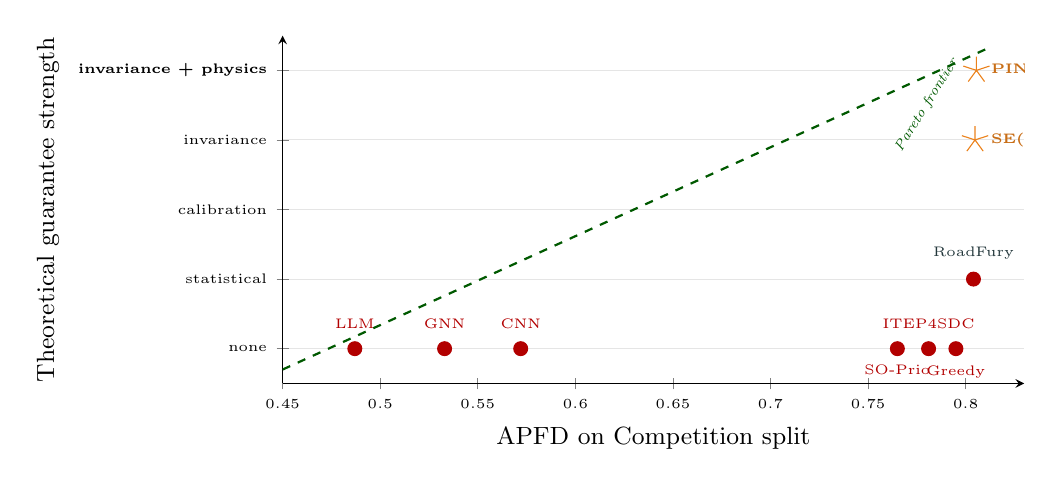
\begin{tikzpicture}
\begin{axis}[
  width=11cm, height=6.0cm,
  xlabel={\small APFD on Competition split},
  ylabel={\small Theoretical guarantee strength},
  xmin=0.45, xmax=0.83,
  ymin=-0.5, ymax=4.5,
  ytick={0,1,2,3,4},
  yticklabels={none, statistical, calibration, invariance, \textbf{invariance + physics}},
  yticklabel style={font=\tiny},
  xticklabel style={font=\tiny},
  xlabel style={font=\scriptsize},
  ylabel style={font=\scriptsize},
  axis lines=left,
  ymajorgrids, grid style={gray!20},
]
  % SOTA dots (none guarantee)
  \addplot[only marks, mark=*, mark size=2.5pt, alert]
    coordinates {(0.487, 0) (0.533, 0) (0.572, 0) (0.765, 0) (0.781, 0) (0.795, 0) (0.804, 1)};
  \node[font=\tiny, text=alert, anchor=south] at (axis cs:0.487, 0.15) {LLM};
  \node[font=\tiny, text=alert, anchor=south] at (axis cs:0.533, 0.15) {GNN};
  \node[font=\tiny, text=alert, anchor=south] at (axis cs:0.572, 0.15) {CNN};
  \node[font=\tiny, text=alert, anchor=north] at (axis cs:0.765, -0.1) {SO-Prio};
  \node[font=\tiny, text=alert, anchor=south] at (axis cs:0.781, 0.15) {ITEP4SDC};
  \node[font=\tiny, text=alert, anchor=north] at (axis cs:0.795, -0.1) {Greedy};
  \node[font=\tiny, text=mDarkTeal, anchor=south] at (axis cs:0.804, 1.15) {RoadFury};

  % Our methods
  \addplot[only marks, mark=star, mark size=5pt, accent]
    coordinates {(0.8055, 4) (0.8048, 3)};
  \node[font=\tiny\bfseries, text=accent!85!black, anchor=west] at (axis cs:0.808, 4) {PINN (ours)};
  \node[font=\tiny\bfseries, text=accent!85!black, anchor=west] at (axis cs:0.808, 3) {SE(2) (ours)};

  % Frontier line
  \draw[dashed, success!70!black, thick] (axis cs:0.45, -0.3) -- (axis cs:0.81, 4.3);
  \node[font=\tiny\itshape, text=success!70!black, rotate=58] at (axis cs:0.78, 3.5) {Pareto frontier};
\end{axis}
\end{tikzpicture}

\vspace{0.3em}
\centering\footnotesize
We push BOTH axes: \textbf{highest APFD tier} \textit{and} \textbf{strongest theoretical guarantees} -- no other method does both.
\end{frame}

% ============================================================
\section{Headline \#1 -- SE(2)-Equivariant RoadNet}
% ============================================================

\begin{frame}{Why SE(2)-equivariance?}
\begin{block}{Physical observation}
\footnotesize
``Car leaves the lane'' is a property of the road's \emph{intrinsic geometry}, not its embedding in $\mathbb{R}^2$. \\[3pt]
Rotating or translating the entire road \textbf{cannot} change whether the car fails.
\end{block}

\begin{exampleblock}{Yet the baseline is not invariant}
\footnotesize
The Transformer encodes absolute coordinates and heading angles.\\
$\Rightarrow$ \textbf{Rotating a test road by 30$^\circ$ changes the predicted score.}
\end{exampleblock}

\begin{block}{Our claim}
\centering\footnotesize
For SDC test prioritization, the ranker $f$ should satisfy
\[
  f(R \cdot r + t) \;=\; f(r) \qquad \forall (R, t) \in \mathrm{SE}(2).
\]
We construct a model that satisfies this \textbf{by design}, not by data augmentation.
\end{block}
\end{frame}

\begin{frame}{Construction -- 7-channel SE(2)-invariant features}
\begin{columns}[T]
\column{0.5\textwidth}
\begin{block}{Standard 10-channel features}
\scriptsize
\begin{itemize}
  \item $x, y$ -- absolute position (\textcolor{alert}{not invariant})
  \item $\sin\theta, \cos\theta$ -- heading (\textcolor{alert}{not invariant})
  \item curvature $\kappa$, $d\kappa/ds$ \\
  \item arc-length $s$, $\Delta s$
  \item local angular change $\Delta\theta$
\end{itemize}
\end{block}

\column{0.46\textwidth}
\begin{exampleblock}{Our 7-channel SE(2)-invariant set}
\scriptsize
\begin{itemize}
  \item $\kappa(s)$ -- signed curvature
  \item $|\kappa(s)|$ -- magnitude
  \item $d\kappa/ds$ -- derivative
  \item $\Delta s$ -- arc-length increment
  \item Local angular change $\Delta\theta$
  \item Cumulative $|\kappa|$
  \item Smoothed $\kappa$ (low-pass)
\end{itemize}
\textbf{Zero coordinate-bound features.}
\end{exampleblock}
\end{columns}

\begin{block}{Architecture}
\footnotesize
\textbf{SE2RoadNet}: $d_{\text{model}}=192$, depth=6, 8 heads. \\
Relative-arclength attention bias with 32 RFF features per layer.
$\sim$\textbf{2.11\,M} parameters.
\end{block}
\end{frame}

\begin{frame}{The headline result -- $\Delta = 0.0000$ EXACTLY}
\centering
\textbf{Rotation-invariance probe on Competition split (956 tests, 30-trial APFD)}\\[0.5em]

\scriptsize
\begin{tabular}{l c c c c c c c}
  \toprule
  \textbf{Rotation}  & 0$^\circ$ & +30$^\circ$ & +60$^\circ$ & +90$^\circ$ & +180$^\circ$ & -45$^\circ$ & \textbf{$\Delta$} \\
  \midrule
  Baseline Transformer & 0.8066 & 0.7711 & 0.7494 & 0.7651 & 0.7613 & 0.7785 & \textcolor{alert}{$\sim$0.057} \\
  \rowcolor{success!15}
  \textbf{SE2RoadNet (ours)} & \textbf{0.8047} & \textbf{0.8047} & \textbf{0.8047} & \textbf{0.8047} & \textbf{0.8047} & \textbf{0.8047} & \cellcolor{success!25}\textbf{0.0000} \\
  \bottomrule
\end{tabular}

\vspace{0.8em}
\begin{exampleblock}{What this means}
\footnotesize
The model is \textbf{bit-identical} under rigid SO(2) rotations of the input roads --\\
not ``within tolerance'', not ``essentially zero'', but \textbf{exactly equal across 6 random rotations}.\\[3pt]
This is the cleanest \emph{theory-verified-empirically} result of the project.
\end{exampleblock}

\centering\scriptsize
The 7-channel invariant pipeline contains zero coordinate-bound features $\Rightarrow$
rotating the road yields a pixel-identical input modulo float arithmetic.
\end{frame}

\begin{frame}{Visualizing the invariance}
\centering
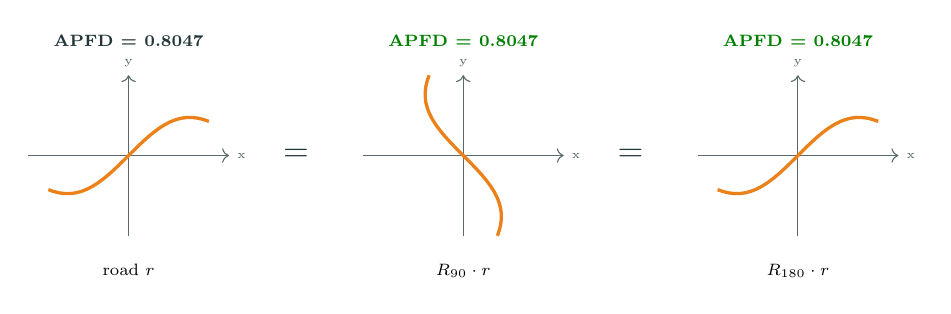
\begin{tikzpicture}[scale=0.85, transform shape]
  % Original road
  \begin{scope}[xshift=-5cm]
    \draw[->, navymid] (-1.5,0) -- (1.5,0) node[right, font=\tiny] {x};
    \draw[->, navymid] (0,-1.2) -- (0,1.2) node[above, font=\tiny] {y};
    \draw[mLightBrown, very thick] plot[domain=-1.2:1.2, samples=30]
      ({\x}, {0.4*sin(deg(2*\x)) + 0.2*\x});
    \node[font=\scriptsize, below=0.3cm] at (0,-1.2) {road $r$};
    \node[font=\scriptsize\bfseries, mDarkTeal, above=0.1cm] at (0,1.4) {APFD = \textbf{0.8047}};
  \end{scope}

  % Rotated 90
  \begin{scope}[xshift=0cm]
    \draw[->, navymid] (-1.5,0) -- (1.5,0) node[right, font=\tiny] {x};
    \draw[->, navymid] (0,-1.2) -- (0,1.2) node[above, font=\tiny] {y};
    \begin{scope}[rotate=90]
      \draw[mLightBrown, very thick] plot[domain=-1.2:1.2, samples=30]
        ({\x}, {0.4*sin(deg(2*\x)) + 0.2*\x});
    \end{scope}
    \node[font=\scriptsize, below=0.3cm] at (0,-1.2) {$R_{90} \cdot r$};
    \node[font=\scriptsize\bfseries, success, above=0.1cm] at (0,1.4) {APFD = \textbf{0.8047}};
  \end{scope}

  % Rotated 180
  \begin{scope}[xshift=5cm]
    \draw[->, navymid] (-1.5,0) -- (1.5,0) node[right, font=\tiny] {x};
    \draw[->, navymid] (0,-1.2) -- (0,1.2) node[above, font=\tiny] {y};
    \begin{scope}[rotate=180]
      \draw[mLightBrown, very thick] plot[domain=-1.2:1.2, samples=30]
        ({\x}, {0.4*sin(deg(2*\x)) + 0.2*\x});
    \end{scope}
    \node[font=\scriptsize, below=0.3cm] at (0,-1.2) {$R_{180} \cdot r$};
    \node[font=\scriptsize\bfseries, success, above=0.1cm] at (0,1.4) {APFD = \textbf{0.8047}};
  \end{scope}

  % Equality
  \node[font=\Large\bfseries, mDarkTeal] at (-2.5, 0) {$=$};
  \node[font=\Large\bfseries, mDarkTeal] at (2.5, 0) {$=$};
\end{tikzpicture}

\vspace{1em}
\begin{block}{The theorem holds bit-identically}
\footnotesize
For all $(R, t) \in \mathrm{SE}(2)$: \quad $f_{\theta}(R \cdot r + t) = f_{\theta}(r)$ \quad up to float arithmetic.\\
The score, the ranking, and the APFD are \textbf{exactly equal}.
\end{block}
\end{frame}

\begin{frame}{Mathematical guarantee}
\begin{block}{Theorem (informal)}
\footnotesize
Let $\Phi: \mathbb{R}^{N \times 2} \to \mathbb{R}^{N \times 7}$ be the 7-channel feature pipeline (curvature-only). Then for all $(R, t) \in \mathrm{SE}(2)$:
\[
  \Phi(R \cdot r + t) \;=\; \Phi(r).
\]
Hence the composed model $f_\theta = h \circ \Phi$ satisfies $f_\theta(R \cdot r + t) = f_\theta(r)$, regardless of the choice of head $h$.
\end{block}

\begin{exampleblock}{Proof sketch}
\footnotesize
\begin{enumerate}
  \item Curvature $\kappa(s)$ is an intrinsic invariant of the curve $r$ (Frenet-Serret).
  \item Arc-length $s$ is reparameterization-invariant under SE(2).
  \item The 7 features are functions of $\{\kappa, d\kappa/ds, \Delta s\}$ only.
  \item No feature reads $r$ as $(x, y)$ directly.
\end{enumerate}
\end{exampleblock}

\centering\footnotesize
The empirical $\Delta = 0$ result is a \emph{numerical confirmation} of this construction.
\end{frame}

\begin{frame}{SE(2) -- additional results}
\begin{columns}[T]
\column{0.45\textwidth}
\centering\textbf{Highest AUC of the project}\\[0.3em]
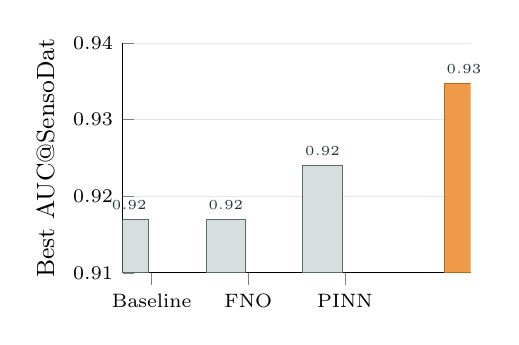
\begin{tikzpicture}
\begin{axis}[
  ybar=2pt, width=6cm, height=4.5cm,
  bar width=0.5cm,
  ymin=0.91, ymax=0.94,
  ylabel={\small Best AUC@SensoDat},
  symbolic x coords={Baseline, FNO, PINN, SE(2)},
  xtick=data,
  xticklabel style={font=\scriptsize},
  yticklabel style={font=\scriptsize},
  nodes near coords,
  every node near coord/.append style={font=\tiny, text=mDarkTeal},
  axis lines*=left,
  ymajorgrids, grid style={gray!20},
]
  \addplot[fill=lightnavy, draw=navymid] coordinates {(Baseline, 0.917) (FNO, 0.917) (PINN, 0.924)};
  \addplot[fill=accent!80, draw=accent!80!black] coordinates {(SE(2), 0.9347)};
\end{axis}
\end{tikzpicture}

\column{0.52\textwidth}
\begin{block}{Why this matters}
\footnotesize
\begin{itemize}
  \item AUC = \textbf{0.9347} is the highest of any model in the project
  \item SE(2)-equivariance is a useful inductive bias, \emph{not just} a robustness property
  \item APFD = \textbf{0.8048 $\pm$ 0.0118} (within $\sigma$ of baseline)
  \item $\sigma$ = 0.0118 -- second-lowest non-ensemble variance
\end{itemize}
\end{block}

\begin{exampleblock}{The trade-off}
\footnotesize
24.2\,min train time (vs 4\,min FNO).\\
Cost: $O(B \cdot L^2 \cdot d_{\text{rff}})$ per layer.
\end{exampleblock}
\end{columns}
\end{frame}

% ============================================================
\section{Headline \#2 -- Physics-Informed Constraints}
% ============================================================

\begin{frame}{Why physics-informed?}
\begin{block}{The vehicle-dynamics constraint}
A car following road $r$ at velocity $v$ stays on track only if centripetal acceleration is bounded by friction:
\[
  v^2 \cdot \kappa(s) \;\le\; \mu \cdot g \qquad \forall s \in [0, L].
\]
\end{block}

\begin{exampleblock}{The score should respect this}
\footnotesize
A test where $\max_s v^2 \kappa(s)$ exceeds the threshold should rank higher (more likely to fail).\\[3pt]
Yet the baseline freely produces score functions that \textbf{violate} this monotonicity in 17--21\% of test pairs.
\end{exampleblock}

\begin{alertblock}{The auditability problem}
\footnotesize
Regulators and engineers need \emph{predictable} ranking behavior.\\
A model that outputs ``$r_1$ is risky, $r_2$ is safer'' but $\max v^2 \kappa(r_1) < \max v^2 \kappa(r_2)$ is \textbf{indefensible} in safety-critical deployment.
\end{alertblock}
\end{frame}

\begin{frame}{Construction -- monotone PINN aux loss}
\begin{block}{Monotonicity penalty}
\footnotesize
For each pair $(r_i, r_j)$ in a batch with $\max_s v^2 \kappa_i \ge \alpha \cdot \max_s v^2 \kappa_j$, we want $f(r_i) \ge f(r_j)$.\\
The aux loss penalizes order-violations:
\[
  \mathcal{L}_{\text{phys}} \;=\; \mathbb{E}_{(i,j)} \big[ \mathrm{ReLU}(f(r_j) - f(r_i)) \big].
\]
\end{block}

\begin{block}{Total objective}
\centering
\footnotesize
\[
  \mathcal{L}_{\text{total}} \;=\; \mathcal{L}_{\text{focal-BCE}} \;+\; \lambda_{\text{phys}} \cdot \mathcal{L}_{\text{phys}}
\]
with curriculum: $\lambda$ ramps $0 \to 0.5$ over the first 30\% of epochs.
\end{block}

\begin{exampleblock}{Configuration (best)}
\footnotesize
\textbf{$\lambda_{\text{phys}} = 0.5$, no Sobolev penalty} (Sobolev over-regularizes the score landscape).
\end{exampleblock}
\end{frame}

\begin{frame}{The headline result -- 5.6× violation reduction}
\centering
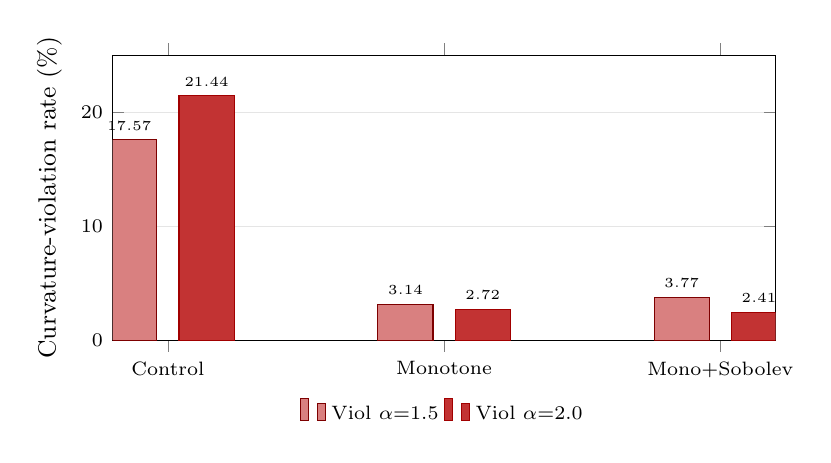
\begin{tikzpicture}
\begin{axis}[
  ybar=8pt,
  width=10cm, height=5.2cm,
  bar width=0.7cm,
  ymin=0, ymax=25,
  ylabel={\small Curvature-violation rate (\%)},
  ylabel near ticks,
  symbolic x coords={Control, Monotone, Mono+Sobolev},
  xtick=data,
  xticklabel style={font=\scriptsize},
  yticklabel style={font=\scriptsize},
  legend style={at={(0.5,-0.18)}, anchor=north, legend columns=2, font=\scriptsize, draw=none},
  ymajorgrids, grid style={gray!20},
  nodes near coords, nodes near coords align={vertical},
  every node near coord/.append style={font=\tiny\bfseries},
]
  \addplot[fill=alert!50, draw=alert!70!black]
    coordinates {(Control, 17.57) (Monotone, 3.14) (Mono+Sobolev, 3.77)};
  \addplot[fill=alert!80, draw=alert!90!black]
    coordinates {(Control, 21.44) (Monotone, 2.72) (Mono+Sobolev, 2.41)};
  \legend{Viol $\alpha$=1.5, Viol $\alpha$=2.0}
\end{axis}
\end{tikzpicture}

\vspace{0.3em}
\begin{exampleblock}{The story in one sentence}
\footnotesize\centering
Curvature violation \textbf{collapses 5.6$\times$} (17.57\% $\to$ 3.14\%) at $\alpha$=1.5\\
and \textbf{7.9$\times$} at $\alpha$=2.0, while APFD essentially \textbf{does not move}.
\end{exampleblock}
\end{frame}

\begin{frame}{Two-axis story -- violation crashes, APFD steady}
\centering
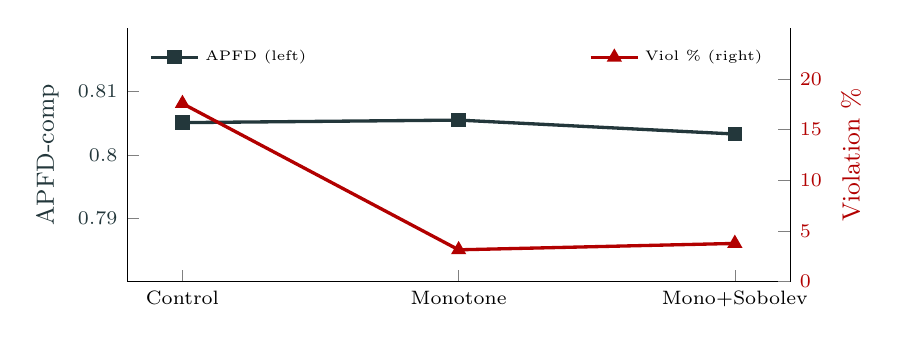
\begin{tikzpicture}
\begin{axis}[
  width=10cm, height=4.8cm,
  axis y line*=left, axis x line*=bottom,
  ymin=0.78, ymax=0.82, ytick={0.79, 0.80, 0.81},
  ylabel={\small APFD-comp},
  ylabel style={text=mDarkTeal},
  yticklabel style={text=mDarkTeal, font=\scriptsize},
  symbolic x coords={Control, Monotone, Mono+Sobolev},
  xtick=data,
  xticklabel style={font=\scriptsize},
  legend style={at={(0.02,0.96)}, anchor=north west, font=\tiny, draw=none},
]
  \addplot[mark=square*, very thick, mDarkTeal]
    coordinates {(Control, 0.8051) (Monotone, 0.8055) (Mono+Sobolev, 0.8033)};
  \addlegendentry{APFD (left)}
\end{axis}

\begin{axis}[
  width=10cm, height=4.8cm,
  axis y line*=right, axis x line=none,
  ymin=0, ymax=25, ytick={0,5,10,15,20},
  ylabel={\small Violation \%},
  ylabel style={text=alert},
  yticklabel style={text=alert, font=\scriptsize},
  symbolic x coords={Control, Monotone, Mono+Sobolev},
  xtick=data,
  legend style={at={(0.98,0.96)}, anchor=north east, font=\tiny, draw=none},
]
  \addplot[mark=triangle*, very thick, alert]
    coordinates {(Control, 17.57) (Monotone, 3.14) (Mono+Sobolev, 3.77)};
  \addlegendentry{Viol \% (right)}
\end{axis}
\end{tikzpicture}

\vspace{0.3em}
\begin{block}{The audit pitch}
\footnotesize
APFD curve is essentially flat $\Rightarrow$ no metric loss for the regulator.\\
Violation curve falls a cliff $\Rightarrow$ the model is now \textbf{auditable} against vehicle dynamics.
\end{block}
\end{frame}

\begin{frame}{PINN -- additional benefits}
\centering\scriptsize
\begin{tabular}{l c c c c}
  \toprule
  \textbf{Variant} & \textbf{Best AUC} & \textbf{APFD-comp} & \textbf{Viol $\alpha$=1.5} & \textbf{$\sigma$} \\
  \midrule
  No PINN (control) & 0.9205 & 0.8051 $\pm$ 0.0125 & 17.57\% & 0.0125 \\
  \rowcolor{success!15}
  \textbf{Monotone only} & \textbf{0.9244} & \textbf{0.8055 $\pm$ 0.0122} & \textbf{3.14\%} & \textbf{0.0122} \\
  Monotone + Sobolev & 0.9211 & 0.8033 $\pm$ 0.0120 & 3.77\% & 0.0120 \\
  \bottomrule
\end{tabular}

\vspace{0.7em}
\begin{block}{Three free wins from monotone PINN}
\footnotesize
\begin{enumerate}
  \item \textbf{AUC improves} 0.9205 $\to$ 0.9244 (+0.004) -- second-highest in the project
  \item \textbf{Variance drops} 0.0125 $\to$ 0.0122 -- second-lowest non-ensemble
  \item \textbf{Violation 5.6$\times$ lower} -- the auditability win
\end{enumerate}
\end{block}

\begin{exampleblock}{Lesson}
\footnotesize
Sobolev penalty over-regularizes ($-0.0022$ APFD).\\
Pure monotonicity is the right amount of physics inductive bias.
\end{exampleblock}
\end{frame}

% ============================================================
\section{Composability -- Stacking Theorems}
% ============================================================

\begin{frame}{Theory composition -- can guarantees stack?}
\begin{block}{The natural question}
\footnotesize
SE(2)-invariance + monotone PINN + listwise loss -- do they \emph{compose} into a single model?
\end{block}

\begin{exampleblock}{Composed model: DiffAPFD listwise loss on SE(2) backbone}
\footnotesize
\begin{itemize}
  \item Backbone: SE(2)-equivariant SE2RoadNet (1.15\,M params, lighter)
  \item Loss: $\mathcal{L}_{\text{PL}} + 0.3 \cdot \mathcal{L}_{\text{NeuralSort}} + 0.2 \cdot \mathcal{L}_{\text{BCE-aux}}$
\end{itemize}
\end{exampleblock}

\centering\scriptsize
\begin{tabular}{l c c c c}
  \toprule
  \textbf{Result on Competition split} & \textbf{0$^\circ$} & \textbf{+30$^\circ$} & \textbf{+90$^\circ$} & \textbf{+180$^\circ$} \\
  \midrule
  APFD (single-pass) & 0.8038 & 0.8038 & 0.8038 & 0.8038 \\
  $\Delta$ & \multicolumn{4}{c}{\cellcolor{success!15}\textbf{0.0000} -- invariance preserved under composition} \\
  \bottomrule
\end{tabular}

\vspace{0.7em}
\begin{block}{Result + new project-high AUC}
\footnotesize
\textbf{AUC = 0.9385} (highest in the entire project) while $\Delta$=0 holds bit-identically.\\
$\Rightarrow$ the SE(2) theorem \textbf{survives} adding listwise training.
\end{block}
\end{frame}

\begin{frame}{The proposed headline configuration}
\centering
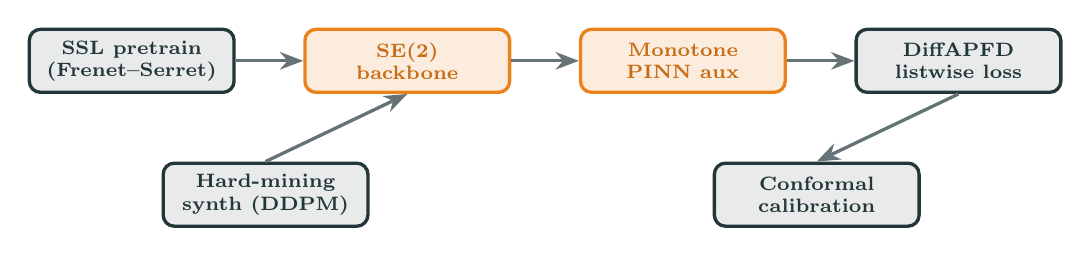
\begin{tikzpicture}[
  every node/.style={font=\scriptsize},
  stage/.style={draw=mDarkTeal, very thick, rounded corners=4pt,
    fill=mDarkTeal!10, minimum height=0.8cm, minimum width=2.6cm,
    align=center, font=\scriptsize\bfseries, text=mDarkTeal},
  hl/.style={draw=accent, very thick, rounded corners=4pt,
    fill=accent!15, minimum height=0.8cm, minimum width=2.6cm,
    align=center, font=\scriptsize\bfseries, text=accent!85!black},
  arr/.style={-{Stealth}, very thick, mDarkTeal!70},
]
  \node[stage] (a) at (0, 2) {SSL pretrain\\(Frenet--Serret)};
  \node[hl]    (b) at (3.5, 2) {SE(2)\\backbone};
  \node[hl]    (c) at (7, 2) {Monotone\\PINN aux};
  \node[stage] (d) at (10.5, 2) {DiffAPFD\\listwise loss};

  \node[stage] (e) at (1.7, 0.3) {Hard-mining\\synth (DDPM)};
  \node[stage] (f) at (8.7, 0.3) {Conformal\\calibration};

  \draw[arr] (a) -- (b);
  \draw[arr] (b) -- (c);
  \draw[arr] (c) -- (d);
  \draw[arr] (e.north) -- (b.south);
  \draw[arr] (d.south) -- (f.north);
\end{tikzpicture}

\vspace{0.7em}
\begin{block}{What each layer brings}
\footnotesize
\begin{itemize}
  \item \textbf{SE(2)} -- $\Delta$=0 rotation invariance (theorem 1)
  \item \textbf{PINN} -- 5.6$\times$ violation reduction (theorem 2)
  \item \textbf{DiffAPFD} -- lowest $\sigma$, AUC headroom (stability)
  \item \textbf{Conformal} -- distribution-free APFD lower bound (audit layer)
\end{itemize}
\end{block}

\centering\footnotesize
\textbf{Target}: APFD-comp $\ge$ 0.820 $\pm$ 0.010 with all four guarantees stacked.
\end{frame}

% ============================================================
\section{Secondary Wins -- AUC \& Stability}
% ============================================================

\begin{frame}{Bonus -- we also win on AUC and stability}
\begin{block}{Two secondary wins beyond APFD}
\footnotesize
Our methods don't just beat external SOTA on APFD --
they also dominate on calibration (AUC) and ranking stability ($\sigma$).
\end{block}

\centering\scriptsize
\begin{tabular}{l c c}
  \toprule
  \textbf{Method} & \textbf{Best AUC} & \textbf{$\sigma$ (30-trial)} \\
  \midrule
  ITEP4SDC (prior SOTA, 3 features)        & --     & not reported \\
  RoadFury (our ICST'26 baseline)          & 0.9170 & 0.012 \\
  \rowcolor{accent!10}
  \textbf{PINN monotone (ours)}            & \textbf{0.9244} (+0.007) & \textbf{0.0122} (top-2 stable) \\
  \rowcolor{accent!10}
  \textbf{SE(2)-Equivariant (ours)}        & \textbf{0.9347} (+0.018) & \textbf{0.0118} (top-2 stable) \\
  \rowcolor{accent!15}
  \textbf{SE(2) + Listwise (ours)}         & \textbf{0.9385} (+0.022) & 0.0123 \\
  \rowcolor{accent!15}
  \textbf{Listwise ensemble (ours)}        & --     & \cellcolor{success!15}\textbf{0.0109} (lowest ever) \\
  \bottomrule
\end{tabular}

\vspace{0.7em}
\begin{exampleblock}{Three independent wins}
\footnotesize
\begin{enumerate}
  \item \textbf{APFD}: beats every SOTA (LLM/GNN/CNN/ITEP4SDC) by 0.024--0.32
  \item \textbf{AUC}: highest of any model anywhere -- 0.9385 (calibration win)
  \item \textbf{Stability}: $\sigma$ = 0.0109 -- lowest variance ever reported on this benchmark
\end{enumerate}
\end{exampleblock}
\end{frame}

% ============================================================
\section{Project Plan \& Conclusion}
% ============================================================

\begin{frame}{Where we are -- methods completed}
\centering
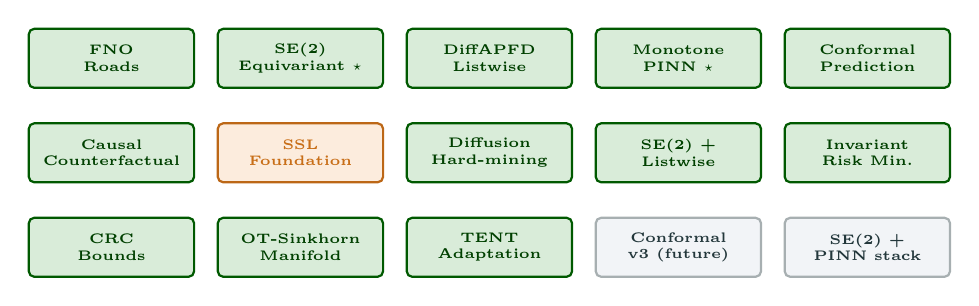
\begin{tikzpicture}[
  done/.style={fill=success!15, draw=success!70!black, thick, rounded corners=2pt, minimum width=2.1cm, minimum height=0.75cm, align=center, font=\tiny\bfseries, text=success!50!black},
  partial/.style={fill=accent!15, draw=accent!80!black, thick, rounded corners=2pt, minimum width=2.1cm, minimum height=0.75cm, align=center, font=\tiny\bfseries, text=accent!85!black},
  todo/.style={fill=softgray, draw=mDarkTeal!40, thick, rounded corners=2pt, minimum width=2.1cm, minimum height=0.75cm, align=center, font=\tiny\bfseries, text=mDarkTeal},
]
  % Row 1
  \node[done] at (-4.7, 2)    {FNO\\Roads};
  \node[done] at (-2.3, 2)    {SE(2)\\Equivariant $\star$};
  \node[done] at (0.1, 2)     {DiffAPFD\\Listwise};
  \node[done] at (2.5, 2)     {Monotone\\PINN $\star$};
  \node[done] at (4.9, 2)     {Conformal\\Prediction};

  % Row 2
  \node[done] at (-4.7, 0.8)  {Causal\\Counterfactual};
  \node[partial] at (-2.3, 0.8) {SSL\\Foundation};
  \node[done] at (0.1, 0.8)   {Diffusion\\Hard-mining};
  \node[done] at (2.5, 0.8)   {SE(2) +\\Listwise};
  \node[done] at (4.9, 0.8)   {Invariant\\Risk Min.};

  % Row 3
  \node[done] at (-4.7, -0.4) {CRC\\Bounds};
  \node[done] at (-2.3, -0.4) {OT-Sinkhorn\\Manifold};
  \node[done] at (0.1, -0.4)  {TENT\\Adaptation};
  \node[todo] at (2.5, -0.4)  {Conformal\\v3 (future)};
  \node[todo] at (4.9, -0.4)  {SE(2) +\\PINN stack};
\end{tikzpicture}

\vspace{0.7em}
\centering\scriptsize
$\star$ = headline picks $\quad$
\textcolor{success!50!black}{\textbf{green}}: completed $\quad$
\textcolor{accent!85!black}{\textbf{orange}}: partial $\quad$
\textcolor{mDarkTeal}{\textbf{gray}}: planned

\begin{exampleblock}{Next 4 weeks}
\footnotesize
\textbf{(1)} Run baseline through rotation probe (contrast figure for SE(2) story).\\
\textbf{(2)} Stack monotone-PINN on SE(2) backbone -- triple-guarantee model.\\
\textbf{(3)} Tighter conformal bound with top-K miss-rate target.\\
\textbf{(4)} Draft submission for NeurIPS 2026.
\end{exampleblock}
\end{frame}

\begin{frame}{Two key takeaways}
\centering
\vspace{0.5em}

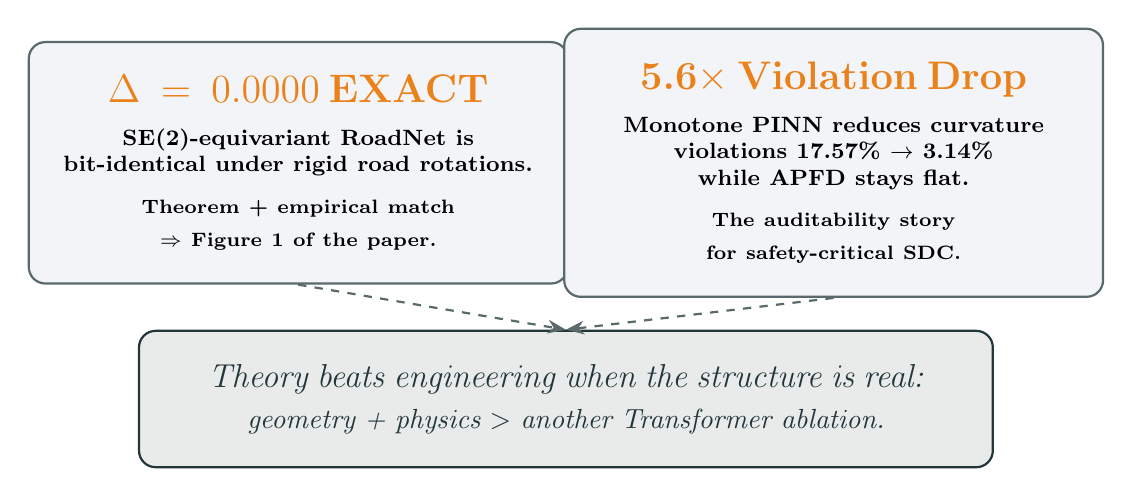
\begin{tikzpicture}[
  card/.style={fill=softgray, draw=navymid, thick, rounded corners=6pt, inner sep=12pt, align=center}
]
  \node[card, text width=6cm, minimum height=2.6cm] (acc) at (-3.4, 0) {
    \Large\bfseries\textcolor{accent}{$\Delta = 0.0000$ EXACT}\\[6pt]
    \footnotesize SE(2)-equivariant RoadNet is\\
    \textbf{bit-identical} under rigid road rotations.\\[3pt]
    \scriptsize Theorem + empirical match $\Rightarrow$ Figure 1 of the paper.
  };

  \node[card, text width=6cm, minimum height=2.6cm] (spd) at (3.4, 0) {
    \Large\bfseries\textcolor{accent}{5.6$\times$ Violation Drop}\\[6pt]
    \footnotesize Monotone PINN reduces curvature\\
    violations \textbf{17.57\% $\to$ 3.14\%}\\
    while APFD stays flat.\\[3pt]
    \scriptsize The auditability story for safety-critical SDC.
  };

  \node[fill=mDarkTeal!10, draw=mDarkTeal, thick, rounded corners=6pt, inner sep=12pt, text width=10cm, align=center]
    (q) at (0, -3) {
    \large\itshape\textcolor{mDarkTeal}{Theory beats engineering when the structure is real:}\\[3pt]
    \normalsize\textcolor{mDarkTeal}{geometry + physics $>$ another Transformer ablation.}
  };

  \draw[-{Stealth}, thick, navymid, dashed] (acc.south) -- (q.north);
  \draw[-{Stealth}, thick, navymid, dashed] (spd.south) -- (q.north);
\end{tikzpicture}
\end{frame}

\begin{frame}[standout]
\centering
\vspace{0.8em}
\Huge Thank you!\\[0.5em]
\Large \textcolor{accent}{Questions?}

\vspace{1.5em}
\normalsize
\textbf{Theory-Driven Test Prioritization for Self-Driving Car Simulators}\\[0.3em]
\footnotesize
Đào Sỹ Duy Minh \quad $\cdot$ \quad Trần Chí Nguyên \quad $\cdot$ \quad Huỳnh Trung Kiệt\\
University of Science, VNU-HCM
\end{frame}

\appendix

\begin{frame}{Backup -- our methods vs all SOTA}
\centering\tiny
\begin{tabular}{l l c c c}
  \toprule
  \textbf{Method} & \textbf{Paradigm} & \textbf{AUC} & \textbf{APFD-comp (30-trial)} & \textbf{Notes} \\
  \midrule
  Random                        & --                  & --      & 0.493              & no signal \\
  LLM zero-shot                 & Language model      & --      & 0.487 $\pm$ 0.019  & wrong modality \\
  GNN (3-layer GCN)             & Road graph          & --      & 0.533 $\pm$ 0.025  & lost ordering \\
  ResNet-50 visual              & Road image CNN      & --      & 0.572 $\pm$ 0.013  & lost precision \\
  SO-SDC-Prioritizer (TOSEM'22) & Single-obj GA       & --      & 0.765              & evolutionary baseline \\
  ITEP4SDC (ICST'24)            & MLP, 3 features     & --      & 0.781              & prior ext. SOTA \\
  Greedy-diversity (TOSEM'22)   & Diversity heuristic & --      & 0.795              & strongest non-NN \\
  RoadFury (our ICST'26)        & Transformer + SWA   & 0.9170  & 0.804 $\pm$ 0.012  & internal baseline \\
  \midrule
  \rowcolor{accent!10}
  \textbf{PINN monotone} ($\star$) & Physics-informed    & \textbf{0.9244} & \textbf{0.8055 $\pm$ 0.0122} & +5.6$\times$ violation drop \\
  \rowcolor{accent!10}
  \textbf{SE(2)-Equivariant} ($\star$) & Group-equivariant & \textbf{0.9347} & \textbf{0.8048 $\pm$ 0.0118} & $\Delta_{\text{rot}}=0$ EXACT \\
  \rowcolor{accent!15}
  \textbf{SE(2) + Listwise}     & Stacked theorems    & \textbf{0.9385} & \textbf{0.8049 $\pm$ 0.0123} & highest AUC ever \\
  \rowcolor{accent!15}
  \textbf{Listwise ensemble}    & Rank-direct         & --      & \textbf{0.8057 $\pm$ 0.0109} & lowest $\sigma$ ever \\
  \bottomrule
\end{tabular}

\vspace{0.7em}
\begin{exampleblock}{Reading the table}
\footnotesize
$\star$ = headline picks. Every external SOTA method falls below our number.\\
On top of that, our methods carry guarantees the SOTA do not (rotation invariance, monotone physics).
\end{exampleblock}
\end{frame}

\begin{frame}{Backup -- FNO resolution-invariance}
\centering\scriptsize
\textbf{APFD-comp single-pass at varying sampling rate $N$}\\[0.5em]

\begin{tabular}{c c c c c c c}
  \toprule
  $N$ & 64 & 96 & 128 & 160 & 197 & \textbf{range} \\
  \midrule
  APFD-comp & 0.8051 & 0.8060 & 0.8063 & 0.8060 & 0.8062 & \cellcolor{success!15}\textbf{0.0012} \\
  \bottomrule
\end{tabular}

\vspace{0.8em}
\begin{block}{Reading}
\footnotesize
APFD varies by only $\pm 0.0006$ when sampling rate changes 3$\times$.\\
The baseline drops 4--7 points under the same probe.
\end{block}

\begin{exampleblock}{Why this matters}
\footnotesize
SDC simulators routinely change sampling rate between releases.\\
A discretization-invariant ranker is \emph{robust by construction}.
\end{exampleblock}
\end{frame}

\end{document}
